\documentclass{scrartcl}

\usepackage[hidelinks]{hyperref}
\usepackage[none]{hyphenat}
\usepackage{graphicx}

\title{When do self-organising Agile game development teams need managing?}
\subtitle{COMP150 -Agile Essay}

\author{Student Number: 1607539}

\begin{document}

\maketitle

\section*{The Scrum Master}

Despite the Agile manifesto \cite {fowler2001agile} itself stating as part of its principles to ``build projects around motivated individuals'', ‘`and to trust them to get the job done'', it still acknowledges the need for a scrum master, not necessarily to act as a manager in the traditional sense, more to ensure adherence to the values and practises of scrum and to remove any impediments to the progress.  The scrum master is responsible for the process used during the software development \cite {larusdottir2016stakeholder}.  Within these subsets of the role are the more traditional management processes: scrum practises may require a level headed methodical approach when requirements are changing late in development, whereas impediments to a sprint may need a more lateral problem solving approach.  Both management and teams jointly manage issues, risks, and solutions \cite {schwaber1997scrum} however in a daily stand up the responsibility falls upon the scrum master.  This pivotal role can be filled by any team member per scrum and as such, consideration must be given when choosing between candidates as to their suitability, not just for responsibility, but also their leadership style and how fitting that is to the sprint tasks at hand.

\section*{Management Styles}

Luckily there already exists a well proven model of managing styles which we can adopt to study the repercussions of each in the context of Agile game development.  Whilst the names and number of terms changes, the extreme values of the scale are usually agreed upon.  From Autocratic as the most dominant, to Laissez-faire which translates to soft touch.  Management styles are distinct from each other in the relative importance of desired goals \cite{fairweather1994goals}.  Leaders and managers are concerned with two aspects of their work.  The first of these aspects we term task accomplishment, organizing activities to perform assigned tasks.  The second aspect we term maintenance of interpersonal relationships, tending to the morale and welfare of the people in the setting \cite {eagly1990gender}.  Each manager's own style is weighted on a gradient towards one of these and it is widely accepted that the optimum management team encapsulates the entire range.  It is important here to differentiate between a management team usually operating over a long period and a single scrum master over a much shorter sprint. 

\section*{An Agile Team}

We should also consider the team members when choosing a way to manage them.  Studies confirm software developers typically fall into specific personality types, the most prominent being ISTJ using the Myers-Briggs Type Indicator (MBTI), introverted, highly rational and analytical `‘thinkers'' rather than `‘feelers'' \cite{wiesche2014relationship}.  Game developers are generally more abstractly artistic and thereby tend to a more extrovert nature.  An extroverted team, can be difficult to manage correctly, however the highly trained, intelligent, and capable nature of software developers counter many of these difficulties.  In a highly trained team for instance, little effort needs to be spent on training; a staple of the more dominant styles.  In fact, with often specialised roles a team may not require any personal management.  The Agile manifesto \cite {fowler2001agile} reflects this in its self-organising guidelines.  Perhaps this is some of the essence of the Scrum methodology?  Not the addition, but the exception of certain techniques and practices, given the software developing prefix.  The role of the product owner defining the rules and parameters of the project, siphoned off in portions through a scrum master to a capable team with the freedom to excel.  Perhaps then it is not the team members that need managing, but the process itself.

\section*{The Sprint}

It is given that dominant forms of supervision best suit inexperienced team members who need direction whilst highly qualified staff will respond better to a Laissez Faire approach.  The analogy of managing a process instead of a person lends itself to the idea that perhaps dominant forms may suit a method where experience is not a factor and the Laissez Faire end of the spectrum where the team's individual expertise must be relied upon.  In which case, we must look at the different stages of a game development project or sprint in terms of freedom of direction and pressure to complete.  On the surface this would seem to be a direct relationship of pressure increasing proportionally over time, however, initially there must be a strong element of control.  In a game development cycle the start is often the planning stage where in lieu of absolute parameters the entire team is concerned with design and creativity.  A wide range of factors (e.g. artistic, emotive, and immersive factors) must be addressed by the requirements engineering effort \cite{callele2005requirements}.  Be it creating the assets, or scripting behaviour, care must be taken to keep the teams vision aligned with the project owner's objective without stifling the creativity of the individuals.  This may seem to warrant a soft touch, but in fact absolute instructions must be given.  The motivational level in respect of Laissez Faire is low because of not interference of management \cite{chaudhry2012impact}, creativity and experience must still be pointed in the required direction.

Over the course of a sprint the need for control decreases.  The role of the scrum master mostly revolves around removing impediments to the process.  With user stories clearly assigned and in progress the Agile principle of trust must be adhered to.  Unless there are changing requirements to the projects parameters a soft touch can now be offered.  This is the point where capable staff thrive and as such, more demanding tasks should be delegated.  As the end of the sprint approaches there must be vigilant oversight to avoid overrunning or under achieving.  As deadlines near, unforeseen circumstances can have drastic implications and correctly identifying and managing these requires the autocratic strength of more dominant techniques. 

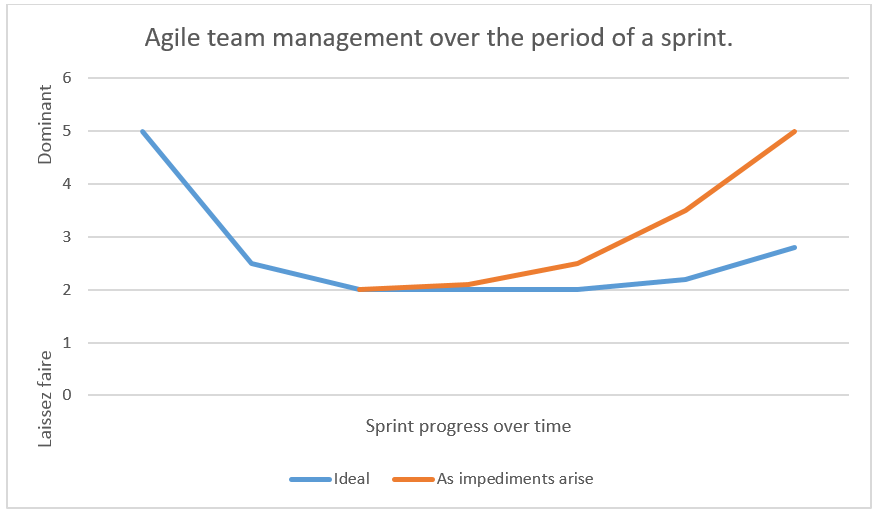
\includegraphics{agile_graph.png}

\section*{Conclusion}

Given that the leadership style of scrum master can be transitioned from one style to another it is possible to optimise an Agile game development team's management through identifying the correct choice for scrum master dependant on the sprint goals and timeframe.  Despite being self-organising by nature, agile teams rely upon guidance beyond user stories, and differing coaching styles must be used to adjust for late-changing requirements and changes in focus and pressures over the course of a sprint.  By utilising the contrasting strengths offered by different management styles the process can be made more efficient, team morale can be improved, and overrunning time frames can be better avoided. 

\bibliographystyle{ieeetran}
\bibliography{references}

\end{document}
